% #############################################################################
% This is Chapter 4
% !TEX root = ../main.tex
% #############################################################################
% Change the Name of the Chapter i the following line
\fancychapter{Architecture}
\cleardoublepage
% The following line allows to ref this chapter
\label{chap:arch}

The fundamental objective of the system was to develop a portable device which enables users and entities to establish safe channels of communication.
A solution was developed on a portable \ac{HSM}, which secures communications between users, saves the owners's sensitive data, such as keys and documents, and performs all security critical operations. This is an easy process for the owner, who does not need to worry about any setup or management, the system is acessible and ready to use, when delivered.
This chapter presents an overview of the developed system, its services, communications protocol and use cases, unconstrained by a specific physical device.

% The system is designed so that each user, either an individual or entity, has it's own physical device.

% -----------------------------------------------------
% -----------------------------------------------------
\section{Overview}\label{chap:arch:overview}

%% COMPONENTS INTRODUCTION %%
The system, pictured in figure~\ref{fig:overview}, is composed of two main components: the physical device, responsible for all operations, and the client software on the user's computer, which provides a simple interface to the user.

\begin{figure}[h]
    \centering
    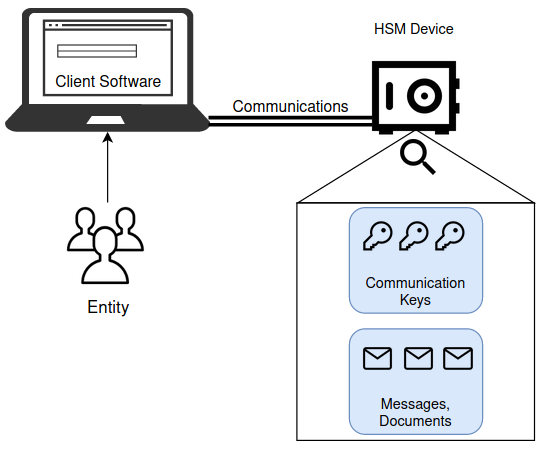
\includegraphics[width=0.75\textwidth]{./Images/overview.png}
    \caption{System Overview}
    \label{fig:overview}
\end{figure}

%% SYSTEM OVERVIEW %%
The client's computer running the software, is connected to the device through a physical connection, used to send and receive data and commands. A simple application for the client's computer was developed to interface with the device.
Using these tools, the entity can signal the device to perform the desired operations.
The implemented services are available inside the device, which stores and manages keys, as well as documents.
If the device is misplaced or stolen, the stored keys and documents are not at risk of being compromised or extracted. The developed software and physical tamper measures ensure it.
Upon receiving their device, each user is only required to plugin it into a power socket, and to their computer using the appropriate cable, and the system is ready to use, through the provided client software.
% All data is either stored in the secure eNVM portion, or in the non-volatile memory, encrypted with an internal \ac{KEK}.

%% SERIAL PORT COMMUNICATIONS INTRODUCTION %%
All data and operations will flow through a serial connection between the client software in the individual's computer and the physical box. A communication protocol which sets the communication rules is defined in the next section.
The serial port connection transmits data one block at a time, each block contains a maximum of 16 bytes.
Data is organized in fields, each field has a fixed number of bytes to hold a specific piece of data.
The protocols are organized in transmissions. One transmission is two messages, one message from the client interface to the device, and another in the reverse direction.

% -----------------------------------------------------
% -----------------------------------------------------
\section{Services Protocols}\label{chap:arch:services}

This next section will describe the services and their communication protocol between the client application and the hardware device. Each service's goal, exchanged information and algorithms are detailed.
Firstly it presents the authentication, then main services, divided in their objective, secure data exchange or new communications.
In the protocol diagrams which will be presented next, data flowing in the same direction consecutively may be shown separately in separate messages. This is only for visibility purposes, in practice, the data is sent together, each in its own field with a defined number of bytes.

% -----------------------------------------------------
% \subsection{Initial State}\label{chap:arch:services:initial-state}

%% DEVICE STATE FROM FABRIC %%
The device will come from fabric configured and prepared with the necessary keys to secure communications.
Before acquiring the device, each entity can provide a list of entities whom they wish to securely communicate. The device will then be delivered to each entity with the necessary keys. This allows owners to begin to communicate immediately, with no setup necessary.
Additionally the device is delivered with the necessary functionality and keys, so all devices can establish new communications with new entities. This provides the flexibility of secure data exchange with a new entity, without having to send the device back to the control station or fabric, to be loaded with the necessary keys.
% depending on two scenarios. In the simpler scenario, the device comes with the symmetric keys already shared and stored in each entities' device.
% In the other scenario, the entities will receive the device with a pair of asymmetric keys, a private and public, generated inside the device from fabric. Each device will have the user's public keys, whom he wishes to communicate. The entity can request whose public keys he wants, before the device is initialized in fabric. This allows the users to share symmetric keys between them, which they can user to begin trading data securely.

Any user needs to be authenticated through a \ac{PIN} number in order to access the system operations. This way, each entity with multiple users can organically handle which users are authorized to handle the system by handing out the corresponding \ac{PIN} number.
The device comes from fabric with a default authentication \ac{PIN}, which is supplied to the owners. It can be changed at any time by an authenticated user.
To authenticate himself to the device, the user sends a \ac{PIN} through the software, the device then compares it to the authentication number securely stored inside it. Once authenticated, the session will be unlocked, and the user will be able to perform operations.

% -----------------------------------------------------
\subsection{Authentication}\label{chap:arch:services:auth}

Before executing any operation the user must authenticate himself to the device.
Figure~\ref{fig:protocol:login} depicts the login protocol.

\begin{figure}[h!]
	\centering
	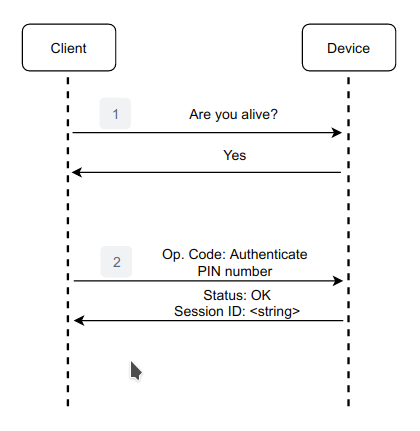
\includegraphics[width=0.50\textwidth]{./Images/authentication.png}
	\caption{Communications protocol to login and change login PIN}
	\label{fig:protocol:login}
\end{figure}

If the user is not authenticated, only the authentication operation is allowed. The communication is initiated by the client interface. It sends the operation code and the login \ac{PIN}.
The device responds with an appropriate failure or success status. If successful, the session will be unlocked, allowing the user access to all other operations.
The user is allowed to change the login \ac{PIN}. The protocol is exactly the same as the login, with the exception that the supplied \ac{PIN} is the new \ac{PIN} which will overwrite the current. The user will receive an error status if not logged in.

% -----------------------------------------------------
\subsection{Secure Data Exchange}\label{chap:arch:services:data-exchange}

The secure data exchange service is responsible for securing communications between users. It grants confidentiality, integrity and authentication to communications.
The communication protocol is illustrated in figure~\ref{fig:protocol:data-exchange}, and consists of two transmissions.
\begin{figure}[h!]
	\centering
	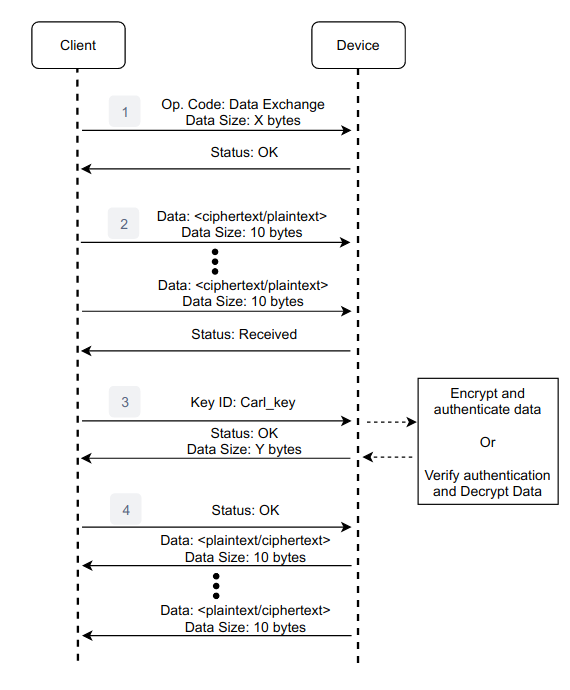
\includegraphics[width=0.60\textwidth]{./Images/data-exchange.png}
	\caption{Communication protocol for the encryption and authentication service using internal HSM keys}
	\label{fig:protocol:data-exchange}
\end{figure}

The first transmission is started by the client sending the operation code and key ID, which identifies the internal \ac{HSM} key used to encrypt and authenticate.
The device returns a status message. If the key ID was invalid or the user is not authenticated, the status is an error.
In the second transmission the client application sends the data length, followed by the data to be encrypted and authenticated internally.
Afterwards, the device start the encryption process and \ac{MAC} generation. When finished, the devices outputs the result length and result data. If there is a processing error, the result length is 0.

The protocol for decryption and encryption is identical. The only difference is in the transmitted data. For the encryption service, the device receives the plaintext data and returns a message with the generated \ac{MAC}, \ac{IV} and encrypted data. For decryption, the device receives the \ac{MAC}, \ac{IV}, ciphertext, and returns the original plaintext.

\begin{equation}
	\label{eq:encrypt-mac}
	E_{key}\{Data, IV\}, MAC_{key}\{IV+E_{key}\{Data, IV\}\}
\end{equation}

The encryption service is pictured in \ref{eq:encrypt-mac}.
First, the plaintext data is encrypted with a symmetric key and a randomly generated \ac{IV}. Next a \ac{MAC} is generated from the concatenated \ac{IV} and ciphertext.

\begin{equation}
	\label{eq:decrypt-mac}
	(MAC_{key}\{IV+Ciphertext\} == MAC) => E_{key}\{Ciphertext, IV\} => Data
\end{equation}

The decryption service is depicted in \ref{eq:decrypt-mac}.
A new \ac{MAC} is generated from the concatenated \ac{IV} and ciphertext received. Then the received and computed {MAC}s are compared. If identical, the data is authenticated, and the ciphertext is decrypted with the same symmetric key used for encryption and the \ac{IV}, to obtain the plaintext.
In the final stage, after the box has finished the cryptographic operations, the device sends the result size to the client, waits for an OK message and returns the result.

% ----------------------------------
\subsection{Qualified Digital Signatures}\label{chap:arch:services:signatures}

The system offers qualified digital signatures, which provide \textbf{non-repudiation} to a piece of data, using a private key generated inside the box. The user sends the data to the box, and the subsequent signature will be returned as pictured in figures~\ref{fig:protocol:signature-generate} and~\ref{fig:protocol:signature-verify}.
The next protocols are relating to the generation and verification of digital signatures.
The communication protocol for generation is represented in figure~\ref{fig:protocol:signature-generate}.

\begin{figure}[h!]
	\centering     %%% not \center
	\subfigure[Generation]{\label{fig:protocol:signature-generate}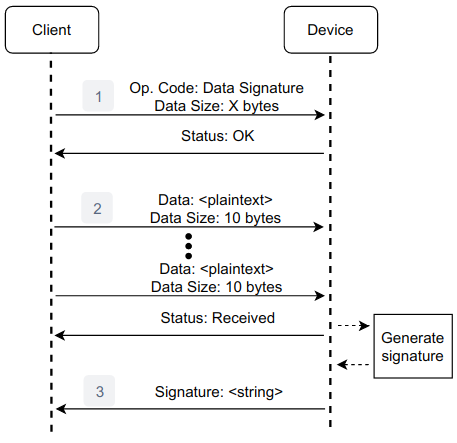
\includegraphics[width=79mm]{Images/signature-generate.png}}
	\subfigure[Verification]{\label{fig:protocol:signature-verify}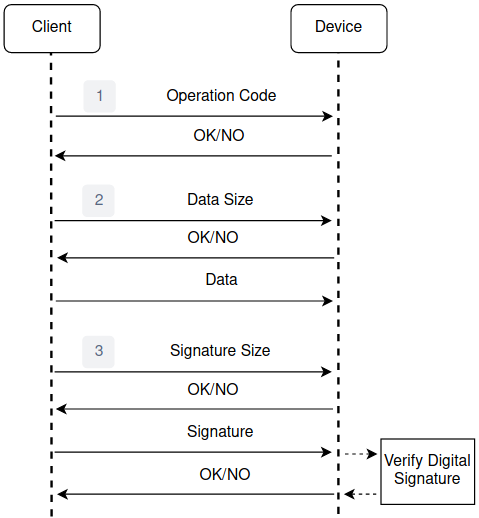
\includegraphics[width=79mm]{Images/signature-verify.png}}
	\caption{Communication protocol for generating digital signatures and verifying the signatures using the internal HSM asymmetric key pair}
\end{figure}

The protocols have one transmission. Messages are separated for readability.
The client application sends the operation code, data length and data to be signed.
The qualified digital signature will be generated using the internal private key and the data. Afterwards the device responds with the signature length and generated signature.
The device will generate the digital signature using the device's private key and a hash function according to the equation \ref{eq:signature-generate}.

\begin{equation}
	\label{eq:signature-generate}
	Sign_{K}\{Hash\{Data\}\}
\end{equation}

The protocol for verifying digital signatures is pictured in figure~\ref{fig:protocol:signature-verify}.
The client sends the operation code, signature length and generated signature, as well as the data length and data from which the signature was generated. The last piece the client sends is the public key of the device where the signature was generated.

After verifying the signature, the device responds with the operation status.
The data is verified using a hash function and the board's \ac{ECC} services, as detailed in \ref{eq:signature-verify}.

\begin{equation}
	\label{eq:signature-verify}
	\{Hash\{Data\}\} == Decrypt_{K_{-1}}\{Signature\}
\end{equation}

The hash is generated from the data using the same hash function as the signer. The result is compared with the value obtained from the decryption of the signature using the signer's public key. The signature is verified if the values are identical.

% -----------------------------------------------------
\subsection{New Communications}\label{chap:arch:services:new-comms}

As introduced before, the device provides the flexibility to establish communications with other entities, even new ones, not previously requested by the user.
The device can also import a new set of keys, provided by the control station.
This way already established channels of communication can be updated in a regular time schedule defined by the entities, in other to maintain secure communications, with the desired entities.

When a user wants to communicate with a new entity, the system provides two convenient solutions. The user can securely contact the control station at any time to request the public information of the other entity, through the secure data exchange service, equivalent to communicating with any other entity.
Then the user needs to send the information through the client software to the device. The new key is generated in the device and made available right away. Then data can be exchanged with the new entity, which must also request the control station for the analogous entity's public information.
This service allows establishing connections with new entities when needed, by way of trusted third party, the control station. 

The system can also be setup with a regular communication update schedule. It grants the flexibility of key revocation when needed, data exchange with new entities, as well as updating communication keys which have reached their expiration date, with no additional complexity to the user, to always safeguard the security of communications.
Each month an entity can hand over a list of the entities it wishes to communicate with to the control station, which will accordingly yield the corresponding key set.
Each entity only needs to forwards the list to the device, and the new keys are immediately stored and ready to be used.
Users can resume communications, same way as before with minimal interruption, with the requested entities.

% -----------------------------------------------------
\subsubsection{ECDH Protocol}\label{chap:arch:services:new-comms:ecdh}

The protocols for the communication management operations are detailed next, namely for symmetric key generation. The protocol to generate a new symmetric key with another entity using asymmetric cryptography is detailed in figure~\ref{fig:protocol:ecdh}.

\begin{figure}[h!]
	\centering
	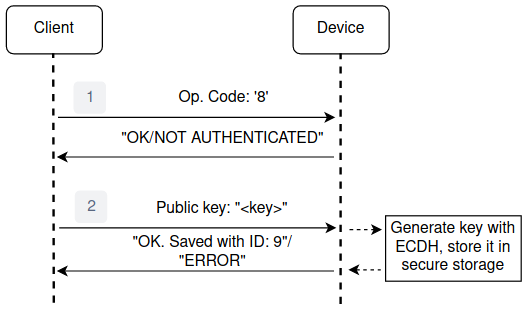
\includegraphics[width=0.60\textwidth]{./Images/ecdh.png}
	\caption{Communication protocol to generate symmetric keys, with the HSM internal private key, and stored them internally}
	\label{fig:protocol:ecdh}
\end{figure}

% The device calls the ECDH algorithm with its private key and the received public key to generate a secret and run it through a key derivation function with the salt value to obtain the new symmetric key. The service's formula is thus:
The user forwards the operation code, public key and salt value to the device.
The device will then generate a symmetric key, using the process in equation \ref{eq:ecdh-kdf}.

\begin{equation}
	\label{eq:ecdh-kdf}
	KDF\{ECDH_{K}\{K^{-1}\}, Salt\}
\end{equation}

A secret is generated from the \ac{ECDH} algorithm, with the device's private key, and another entity's public key. The same secret can be generated with the device's public key and the other entity's private key. 
This secret is run through a key derivation function in conjunction with a salt which can be public, to generate a symmetric key. If both entities generate the same secret and agree on the same salt value, the generated key is identical.

The new key is then stored in non-volatile memory encrypted with the dedicated symmetric encryption key for storage, saved in its PUF slot.
A new unique ID is generated for the key, which is stored alongside the key in memory. This ID is returned to the user along with the operation success status.

% -----------------------------------------------------
\subsubsection{Import Keys Protocol}\label{chap:arch:services:new-comms:import}

This section details the protocol to import a list of encrypted symmetric keys, into the device.
The imported keys must be encrypted with a preset symmetric key, stored inside the device, using \ac{AES} \ac{CTR} mode and authenticated with \ac{HMAC}. This service is useful so a central management section with a similar device can distribute keys to the enrolled entities, on a regular schedule, such as monthly.
The protocol for the service is pictured in figure \ref{fig:protocol:import-keys}.

\begin{figure}[h!]
	\centering
	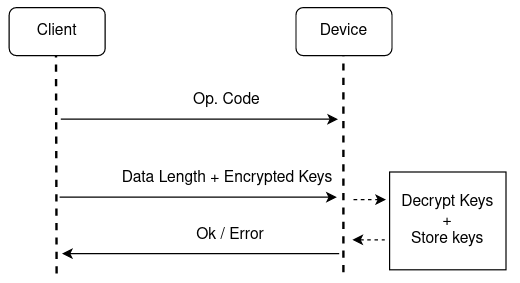
\includegraphics[width=0.60\textwidth]{./Images/import-keys.png}
	\caption{Communication protocol to import encrypted symmetric keys, and store them encrypted in the HSM's memory}
	\label{fig:protocol:import-keys}
\end{figure}

The only transmission consists in the client sending the operation code, keys length and key data. Then, the device decrypts and authenticates the keys using a predefined symmetric key stored in a secure PUF slot. The protocol used is the same for secure data exchange described in the previous section.

Each key consists of 1 byte for its ID, 1 byte for its size and remaining bytes for the key data.
The decrypted list of keys is encrypted and authenticated again, using the same algorithms with a dedicated symmetric key for storage in memory. The ciphertext, randomly generated IV and ciphertext length are stored in memory. To provide authentication and thus protection against tampering, a \ac{MAC} is generated from the three pieces of data and stored in secure storage, separate from the keys and IV.
In order to fetch a stored symmetric key to use in one of the implemented services, the \ac{MAC} is generated and compared to the existing. If identical, the keys can be decrypted from memory and a specific key identified through ID.

% When a symmetric key is revocated, due to reaching its expiration date, or from being compromised, entities can generate a new one, using the aforementioned procedure, with an additional parameter for the key derivation function, to generate a completely new and unique key.
% Import
% Generate

% Supported management operations include generation of new symmetric keys for communication and revocation of existing keys saved in the device, if communications are suspected to be compromised.
% These operations are only available in the scenario where each device has a pair of asymmetric keys, and there is a protocol in place to distribute public keys.

% An entity receives their device, prepared to communicate with other entities, and a list of information of other entities, available to create communications. This information, namely the entities public key, can be imported into the device to generate new keys.
% After the key is imported, a secure connection with a new entity can be established, by sharing symmetric keys.
% In order for an entity to communicate with a another entity, with no previously established communications, their device will generate a new symmetric key and store it in secure storage, or in non-volatile memory, encrypted with the device's public key.

% -----------------------------------------------------
\section{Summary}\label{chap:arch:summary}

This section described the system's functionalities in a practical approach with examples for end users.
The system grants secure communications between any number of users, as soon as they receive the device, without overloading the users with convoluted tasks or responsibilities.
It is very flexible in allowing entities to manage the authorized user's to their devices and with whom they wish to communicate, by offloading this management component and responsibility to a trusted control station.
